\chapter{Next Steps and Moving to 2D\label{ch:5_2DGKP}}


In the previous chapter, we presented the results of our experiments with a fluxonium in a 3D cavity. We demonstrated a tunable dispersive shift between the qubit and the storage resonator via bosonic mode threading and characterized the various components of our system. In doing so, we discovered that the lifetime of the storage mode was \textit{significantly} lower than expected (as compared to its bare value) whenever the qubit chip was inserted into the resonator package. After many rounds of experimentation and testing, we were ultimately able to attribute this effect to two main sources: (i) the storage mode's coupling to the lossy qubit flux line; and (ii), its participation in spurious slotline modes of the 3D superconducting package. While the former issue could in principle be solved via clever microwave engineering and filtering, the latter unfortunately is intrinsic to our 3D design and not easily remedied. As we came to learn, it is generally difficult to integrate fast-flux into a 3D cavity while also maintaining the cavity coherence. 

There are certain approaches that have been proposed and implemented in the literature that work towards integrating fast-flux in 3D. One such example is the magnetic hose from Refs. \cite{gargiulo2021fast,valadares2023demand}. Here, the authors route flux from an external coil to a tunable transmon qubit in a 3D superconducting package using a ``hose'' composed of concentric aluminium and mu-metal layers. In the experiment of Ref. \cite{valadares2023demand} specifically, this is done for the purpose of bosonic cQED, and the authors demonstrate that the lifetime of their 3D storage resonator is not limited by their flux delivery mechanism. Unfortunately, however, the design and implementation of a magnetic hose is quite painstaking, and would require a full redesign of both the cavities and the fluxonium chips that were presented in Ch. \ref{ch:4_3DGKP}. Other designs have also been proposed recently, e.g. Ref. \cite{hutin2024monitoring} or Ref. \cite{maiti2024ancilla}, which both rely on some form of on-chip distributed-element microwave filtering to prevent losses from the flux line at the frequency of the storage. Despite requiring more advanced microwave engineering in design, these approach seem promising for integrating fast-flux in 3D while maintaining the storage resonator lifetime. 

In our case, however, after discovering the root cause of our storage coherence issues and identifying various avenues to proceed from there, we decided to forgo the 3D architecture entirely. This was in part due to the time and difficulty of implementing fast-flux delivery in 3D (which, as highlighted above, is a difficult project in of itself); but it was also a choice we made consciously, motivated by the idea of moving our experiments to 2D. Over the course of our 3D-GKP project, we ended up developing an entirely separate but novel way to do GKP error correction in 2D, using a microwave-activated coupler to generate faster conditional displacements. This 2D project, first proposed using a transmon control qubit and later a fluxonium, represents an improvement over the ``direct dispersive'' approach we took in our 3D-GKP project in most ways. As such, we decided that moving to 2D is a more promising long term path towards building extensible GKP error correction systems. 

In this chapter, we present three of our proposals for implementing GKP error correction in 2D. Within our bosonic subgroup in EQuS, we refer to these as the ``RAT'' (see Ch. \ref{sec:5_RAT}), the ``RAF'' (see Ch. \ref{sec:5_RAF}), and the ``2D dispersive'' (see Ch. \ref{sec:5_2D_Disp}) approaches, respectively\footnote{The meaning behind these names will become apparent shortly!}. We will go through the basic theory for all three approaches and discuss high-level results: in particular, we have already completed designs for the RAF and 2D dispersive projects, which are currently being fabricated as of this writing. 

Here, my aim is give a broad overview to our upcoming 2D experiments; however, more details and a discussion of the careful design and simulation considerations taken can be found in the SM thesis of Shantanu Jha. 
\clearpage


\section{The Asymmetrically-Threaded-SQUID Coupler \label{sec:5_RAT}}

The core insight that motivated our investigation into GKP error correction in 2D was that we can use an Asymmetrically-Threaded SQUID (ATS) as a coupler element to realize the desired ``three-wave mixing'' conditional displacement term that underpins all GKP QEC schemes. The ATS is a superconducting dipole element consisting of a symmetric SQUID shunted by an inductor, as shown in Fig. \ref{fig:5_ats_spectrum}(a); the two resulting flux loops in the circuit are then typically biased \textit{asymmetrically} \cite{lescanne2020exponential, berdou2023one}. In practice, the inductor is realized using an array of Josephson junctions and so the circuit itself is similar to that of a gradiometric SNAIL \cite{miano2022frequency}; it was also recently referred to as the Linear Inductive Coupler when biased symmetrically \cite{maiti2024ancilla}. Despite these various names, we will refer to the actual dipole element as an ATS throughout our work, irrespective of its bias point. 

\begin{figure}[h]
    \centering
    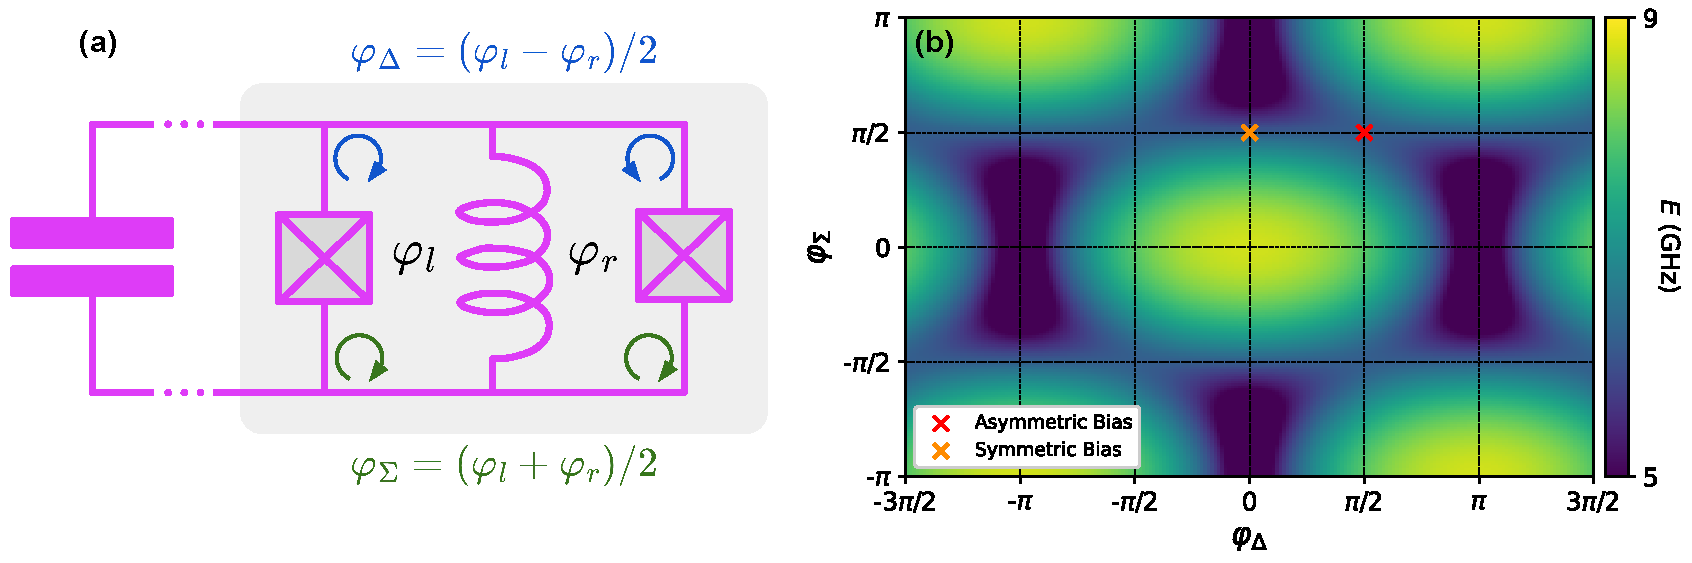
\includegraphics[width=\linewidth]{Figures/5/ats_spectrum.pdf}
    \caption{\textbf{(a)} Circuit diagram for the ATS dipole element (shaded in gray) which consists of a symmetric SQUID shunted by an inductor. The left/right loops are threaded by fluxes $\varphi_l$/$\varphi_r$ respectively, giving rise to common and differential fluxes $\varphi_\Sigma$ and $\varphi_\Delta$. When the ATS is connected to a capacitor, it forms a mode. \textbf{(b)} Fundamental frequency of the ATS mode vs. flux $(\varphi_\Sigma, \varphi_\Delta)$ using parameters $E_L/h = 60$ GHz, $E_J/h = 30$ GHz, and $E_C/h = 80$ MHz.}
    \label{fig:5_ats_spectrum}
\end{figure}

\noindent To begin our exploration of the ATS, let's consider its potential energy, which is given by:
\begin{equation}
    \hat{U}_b = \frac{1}{2}E_L \bigg(\hat{\varphi} + \frac{C_r\varphi_r - C_l\varphi_l}{C_\Sigma}\bigg)^2 - E_{J,l}\cos\!\bigg(\hat{\varphi} + \frac{C_r}{C_\Sigma}[\varphi_l + \varphi_r]\bigg) - E_{J,r}\cos\!\bigg(\hat{\varphi} - \frac{C_l}{C_\Sigma}[\varphi_l + \varphi_r]\bigg)
\end{equation}
Here, we have used the method of Ref. \cite{you2019circuit} to write the potential in terms of its irrotational variable $\hat{\varphi}$, which is the correct approach for time-varying external fluxes; the expression is thus somewhat different from the original description of the ATS in Ref. \cite{lescanne2020exponential}. We have left and right junctions with energies $E_{J, l/r}$, inherent capacitances $C_{l/r}$, and external fluxes $\varphi_{l/r}$ respectively. At this point, we can define the effective $E_J = (E_{J,l} + E_{J,r})/2$ and asymmetry $\Delta E_J = (E_{J,l} - E_{J,r})/2$, and transform to sum and difference coordinates $\varphi_{\Sigma/\Delta} = (\varphi_l \pm \varphi_r)/2$.  Ideally, we would like the junctions to be perfectly symmetric; in practice the asymmetry can be minimized to about $1\%$ of $E_J$. While this is important to keep track of, we will here set $\Delta E_J \to 0$ in the rest of the theory that follows. Thus, $E_{J,l} = E_{J,r} = E_J$ and $C_l = C_r = C$, with $C_\Sigma = C_l + C_r$. We can therefore simplify the complicated expression above and write the potential as:
\begin{equation}
\hat{U}_b(\hat{\varphi}) = \frac{1}{2}E_L(\hat{\varphi} - \varphi_\Delta)^2 - 2E_J \cos(\varphi_\Sigma)\cos(\hat{\varphi})
\end{equation}
In what follows, we will typically keep the differential flux $\varphi_\Delta$ constant and only modulate the common flux $\varphi_\Sigma = \varphi_\Sigma(t)$. Therefore, we can perform a gauge transformation to move the now DC flux $\varphi_\Delta$ to the cosine via $\hat{\varphi} \mapsto \hat{\varphi} + \varphi_\Delta$. This finally get us back to the familiar expression
\begin{equation}
\hat{U}_b(\hat{\varphi}) = \frac{1}{2}E_L\hat{\varphi}^2 - 2E_J \cos(\varphi_\Sigma)\cos(\hat{\varphi} + \varphi_\Delta)
\end{equation}
that can be found in Refs. \cite{lescanne2020exponential, berdou2023one}. We will use this throughout the rest of this chapter.

As shown in Fig. \ref{fig:5_ats_spectrum}(b), when the ATS is connected to a capacitance, the resulting mode has a fundamental frequency that is doubly periodic in $\varphi_\Sigma$ and $\varphi_\Delta$, forming an `egg-carton' potential as it is sometimes referred to. There are two typical operating points for the ATS:

\begin{itemize}
    \item \textbf{Asymmetric bias point:} $(\varphi_\Sigma, \varphi_\Delta) = (\pi/2, \pi/2)$, corresponding to $\varphi_l = \pi$ and $\varphi_r = 0$. This is the standard operating point for the ATS. By modulating the sum flux around this bias, i.e. $\varphi_\Sigma(t) = \pi/2 + \epsilon(t)$, we get the following time-dependent potential for the ATS dipole:
    \begin{equation}
        \hat{U}_b(\hat{\varphi}) = \frac{1}{2}E_L \hat{\varphi}^2 - 2E_J \sin[\epsilon(t)]\sin(\hat{\varphi})
    \end{equation}
\item \textbf{Symmetric bias point:} $(\varphi_\Sigma, \varphi_\Delta) = (\pi/2, 0)$, corresponding to $\varphi_l = \varphi_r = \pi/2$. Biasing here gives us:
\begin{equation}
        \hat{U}_b(\hat{\varphi}) = \frac{1}{2}E_L \hat{\varphi}^2 - 2E_J \sin[\epsilon(t)]\cos(\hat{\varphi})
    \end{equation}
\end{itemize}
%%%%%%%%%%%%%%%%%%%%%%%%
\subsection{The Resonator-ATS-Transmon (RAT)}

Our first approach to faster GKP error correction was developed using the ATS as a coupler element between a storage resonator and a transmon control qubit. We name this the RAT. The basic idea relies on black-box quantization (cf. Ch. \ref{ch:3_cQED}) between the three modes $\hat{a}_0$, $\hat{b}_0$, and $\hat{q}_0$ for the resonator, ATS, and transmon respectively. The bare transmon Hamiltonian is:
\begin{equation}
\hat{H}_{q, 0} = 4E_{C,q}\hat{n}_q^2 - E_{J,q}\cos(\hat{\theta}) = \omega_{q,0}\,\hat{q}_0^\dagger \hat{q}_0 - \Big[E_{J,q}\cos(\hat{\theta}) + \frac{1}{2}E_{J,q} \hat{\theta}^2\Big] 
\end{equation}
where we write the mode $\hat{q}_0$ in terms of the transmon charge $\hat{n}_q$ and phase-drop $\hat{\theta}$. For the ATS, it is:
\begin{equation}
\hat{H}_{b,0} = 4E_C \hat{n}^2 + \hat{U}_b(\hat{\varphi}) = \omega_{b,0}\hat{b}_0^\dagger \hat{b}_0 - 2E_J \cos(\varphi_\Sigma)\cos(\hat{\varphi} + \varphi_\Delta)
\end{equation}
in terms of the ATS charge operator $\hat{n}$ and phase-drop $\hat{\varphi}$. Finally, for the storage we have $\hat{H}_{a, 0} = \omega_{a,0}\hat{a}_0^\dagger \hat{a}_0$. If we take the modes to be linearly coupled (e.g. via capacitive coupling) in series, i.e. resonator $\leftrightarrow$ ATS $\leftrightarrow$ transmon, then the total Hamiltonian has a \textit{linear} part:
\begin{equation}
\hat{H}_{\rm lin, 0} = \omega_{a,0}\hat{a}_0^\dagger \hat{a}_0 + \omega_{b,0}\hat{b}_0^\dagger \hat{b}_0 + \omega_{q,0}\hat{q}_0^\dagger \hat{q}_0 - g_{ab}(\hat{a}_0 - \hat{a}_0^\dagger)(\hat{b}_0 - \hat{b}_0^\dagger) - g_{qb}(\hat{b}_0 - \hat{b}_0^\dagger)(\hat{q}_0 - \hat{q}_0^\dagger)
\end{equation}
Following black-box quantization, we can diagonalize $\hat{H}_{\rm lin, 0}$ as a system of normal modes $\hat{a}$ (storage-like), $\hat{b}$ (buffer-like), and $\hat{q}$ (qubit-like). In this basis $\hat{H}_{\rm lin} = \omega_a \hat{a}^\dagger\hat{a} + \omega_b \hat{b}^\dagger\hat{b} + \omega_q \hat{q}^\dagger\hat{q}$, where $\omega_a$, $\omega_b$, and $\omega_q$ are the normal mode frequencies. We can also rewrite the bare modes in this normal mode basis via a linear transformation:
\begin{align}
\hat{\theta} &= \theta_{q, 0}(\hat{q}_0 + \hat{q}_0^\dagger) = \theta_q(\hat{q} + \hat{q}^\dagger) + \theta_b(\hat{b} + \hat{b}^\dagger) + \theta_a(\hat{a} + \hat{a}^\dagger) \\
\hat{\varphi} &= \phi_{b, 0}(\hat{b}_0 + \hat{b}_0^\dagger) = \phi_q(\hat{q} + \hat{q}^\dagger) + \phi_b(\hat{b} + \hat{b}^\dagger) + \phi_a(\hat{a} + \hat{a}^\dagger)
\end{align}
Here, $\theta_i$ denotes the participation of mode $i$ in the phase across the Josephson junction in the transmon, while $\phi_i$ is the participation in the phase across the ATS. In total, we have
\begin{equation}
\hat{H} = \sum_{c = \{a, b, q\}}\omega_c \hat{c}^\dagger\hat{c} - \Big[E_{J,q}\cos(\hat{\theta}) + \frac{1}{2}E_{J,q} \hat{\theta}^2\Big] - 2E_J \cos(\varphi_\Sigma)\cos(\hat{\varphi} + \varphi_\Delta)
\end{equation}
as the Hamiltonian for the full resonator-ATS-transmon system written in the ``black-box quantization'' basis (i.e. of the normal modes of the linearized circuit). 

With the Hamiltonian written down, let's now see how to get conditional displacements out of it. We park the ATS at its standard asymmetric bias point $(\varphi_\Sigma, \varphi_\Delta) = (\pi/2, \pi/2)$ and modulate $\varphi_\Sigma(t) = \pi/2 + \epsilon(t)$ about this. The ATS potential takes on the form $\sin[\epsilon(t)]\sin(\hat{\varphi})$, and so we can Taylor expand $\sin[\epsilon(t)] \approx \epsilon(t)$ and $\sin(\hat{\varphi}) \approx \hat{\varphi} - \hat{\varphi}^3/6$ in anticipation of making a rotating-wave approximation. We can also truncate the transmon potential to a Duffing oscillator, considering only the leading fourth-order nonlinearity. These approximations give us
\begin{equation}
\hat{H} = \sum_{c = \{a, b, q\}}\omega_c \hat{c}^\dagger\hat{c} - \frac{E_{J,q}}{24}\hat{\theta}^4 - 2E_J \epsilon(t)\hat{\varphi} + \frac{1}{3}E_J\epsilon(t)\hat{\varphi}^3
\end{equation}
We go into a rotating frame for each of the modes $\hat{c} \mapsto \hat{c} e^{-i\tilde{\omega}_c t}$ where we set the frequency $\widetilde{\omega}_c = \omega_c - \theta_{c}^{2} \big[\theta_{a}^{2} + \theta_{b}^{2} + \theta_{q}^{2}\big]/2$ to cancel out the frequency normalizations that arise from the transmon nonlinearity. In this frame, we get
\begin{align}
\begin{split}
\hat{H} &= \hat{H}_{cc} - \frac{E_{J,q}}{24}\Big[\theta_q(\hat{q}e^{-i\tilde{\omega}_q t} + \hat{q}^\dagger e^{i\tilde{\omega}_q t}) + \theta_b(\hat{b}e^{-i\tilde{\omega}_b t} + \hat{b}^\dagger e^{i\tilde{\omega}_b t}) + \theta_a(\hat{a}e^{-i\tilde{\omega}_a t} + \hat{a}^\dagger e^{i\tilde{\omega}_a t})\Big]^4 \\&\quad- 2E_J\epsilon(t)\Big[\phi_q(\hat{q}e^{-i\tilde{\omega}_q t} + \hat{q}^\dagger e^{i\tilde{\omega}_q t}) + \phi_b(\hat{b}e^{-i\tilde{\omega}_b t} + \hat{b}^\dagger e^{i\tilde{\omega}_b t}) + \phi_a(\hat{a}e^{-i\tilde{\omega}_a t} + \hat{a}^\dagger e^{i\tilde{\omega}_a t})\Big]\\ &\quad + \frac{1}{3}E_J\epsilon(t)\Big[\phi_q(\hat{q}e^{-i\tilde{\omega}_q t} + \hat{q}^\dagger e^{i\tilde{\omega}_q t}) + \phi_b(\hat{b}e^{-i\tilde{\omega}_b t} + \hat{b}^\dagger e^{i\tilde{\omega}_b t}) + \phi_a(\hat{a}e^{-i\tilde{\omega}_a t} + \hat{a}^\dagger e^{i\tilde{\omega}_a t})\Big]^3
\end{split}
\end{align}
where $\hat{H}_{cc} = \sum (\omega_c - \tilde{\omega}_c)\hat{c}^\dagger\hat{c}$ will cancel out when the terms are expanded. At this point our task involves sorting through the various pumped nonlinear terms and keeping only the ones that survive the RWA. We set $\epsilon(t) = \epsilon_p \sin(\omega_p t)$ with $\omega_p = \tilde{\omega}_a$, picking out terms that rotate at the (renormalized) storage frequency. Luckily we can do the oscillator expansion, normal ordering, and RWA all numerically using SymPy. The final effective Hamiltonian
\begin{align}
\begin{split}
\hat{H}_{\rm eff} &= \frac{K_a}{2}{{a}^\dagger}^{2} {a}^{2} + \frac{K_b}{2}{{b}^\dagger}^{2} {b}^{2} + \frac{K_q}{2}{{q}^\dagger}^{2} {q}^{2} + \frac{\chi_{ab}}{2}\hat{a}^\dagger\hat{a}\hat{b}^\dagger\hat{b} + \frac{\chi_{aq}}{2} \hat{a}^\dagger\hat{a}\hat{q}^\dagger\hat{q} + \frac{\chi_{qb}}{2} \hat{q}^\dagger\hat{q}\hat{b}^\dagger\hat{b} \\
&\quad + g_{\rm CD}{{q}^\dagger} {q}\big(\hat{a} + \hat{a}^\dagger\big) + g_{\rm disp} \big(\hat{a}+\hat{a}^\dagger\big) + g_a\big[{{a}^\dagger} {a}^{2} + {{a}^\dagger}^{2} {a}\big] + g_b {{b}^\dagger} {b}\big(\hat{a} + \hat{a}^\dagger\big) 
\end{split}
\end{align}
has many terms that we can categorize as follows. We have Kerr nonlinearities for all three modes $K_x = -E_{J, q}\theta_{x}^{4} / 2$ and cross-Kerr dispersive shifts $\chi_{xy} = -2E_{J, q}\theta_{x}^{2} \theta_{y}^{2}$. Next, we have the desired conditional displacement $g_{\rm CD} = E_J\epsilon_{p} \phi_{a} \phi_{q}^{2}$ and an unconditional displacement $g_{\rm disp} = E_J\epsilon_p\big[\phi_a^3 +\phi_{a} \phi_{q}^{2} + \phi_{a} \phi_{b}^{2} - 2\phi_a\big]/2$. Finally, we also have two spurious nonlinear terms associated with the storage and ATS mode: $g_a = E_J\epsilon_{p} \phi_{a}^{3}/2$ and $g_b = E_J\epsilon_{p} \phi_{a}\phi_{b}^{2}$. The qubit anharmonicity $K_q$ should not affect the oscillator dynamics, and just provides the requisite nonlinearity for control. Furthermore, if the ATS is never strongly populated $\ev{\hat{b}^\dagger\hat{b}} \approx 0$, we can further simplify to just:
\begin{equation}
\hat{H}_{\rm eff} = \frac{\chi_{aq}}{2} \hat{a}^\dagger\hat{a}\hat{q}^\dagger\hat{q} + \frac{K_a}{2}{{a}^\dagger}^{2} {a}^{2} + g_{\rm CD}{{q}^\dagger} {q}\big(\hat{a} + \hat{a}^\dagger\big) + g_{\rm disp} \big(\hat{a}+\hat{a}^\dagger\big) + g_a\big[{{a}^\dagger} {a}^{2} + {{a}^\dagger}^{2} {a}\big]
\label{eq:5_FCD_full_hamiltonian}
\end{equation}
Overall, we have the desired conditional displacement term, along with several additional unwanted terms that we will now discuss how to cancel out. Note that all drive-activated terms are proportional to the flux pump envelope $\epsilon_p = \epsilon_p(t)$, which we can pulse to activate the desired interactions. 

\subsection{Conditional Displacements with the RAT}

It turns out that we can cancel many of the unwanted terms above using an echo protocol reminiscent of the echoed conditional displacement (ECD) from Ref. \cite{eickbusch2022fast} that we reviewed in Ch. \ref{ch:2_QEC}. To see how, let's consider a simplified version of Eq. \eqref{eq:5_FCD_full_hamiltonian} with just the CD term and the dispersive shift. We also truncate the transmon to a two-level qubit $\hat{q}^\dagger\hat{q} \to \hat{\sigma}_z$ and thus have:
\begin{equation}
\hat{H}(t) = \frac{\chi}{2}\hat{a}^\dagger\hat{a}[z(t)\hat{\sigma}_z]   + \Big[g_{\rm CD}(t)\hat{a}^\dagger + g_{\rm CD}^\ast(t)\hat{a}\Big]z(t)\hat{\sigma}_z
\label{eq:5_FCD_simplified_hamiltonian}
\end{equation}
Here we have included a fictitious qubit state parameter $z(t) = \ev{\sigma_z(t)}$ that tells us when to perform $\pi$-pulses \cite{eickbusch2022-ECD}, and also explicitly highlight the time-dependence $g_{\rm CD}(t)$ controlled via the flux pump. We can then solve the Schr\"odinger equation $i\partial_t\hat{U} = \hat{H}(t)\hat{U}$ in terms of a parameterized ansatz $\hat{U}(t)$. We find the same ansatz and solution as Ref. \cite{eickbusch2022-ECD}: 
\begin{equation}
    \hat{U}(t) = \exp(i\theta \hat{\sigma}_z / 2)\,\exp\!\Big[\hat{a}^\dagger(\gamma + \delta \hat{\sigma}_z) - \hat{a}(\gamma^\ast + \delta^\ast \hat{\sigma}_z)\Big]\exp(i\phi\hat{a}^\dagger\hat{a}\hat{\sigma}_z)
\end{equation}
where $\theta(t), \gamma(t), \delta(t), \phi(t)$ correspond to a qubit rotation, cavity displacement and conditional displacement, and a qubit-selective cavity rotation. Plugging in Eq. \eqref{eq:5_FCD_simplified_hamiltonian} and solving the Schr\"odinger equation, it turns out we can actually find a solution:
\begin{align}
    \begin{split}
        \theta(t) & = +2 \int_0^t d\tau \mathrm{Re}[g_{\rm CD}^*(\tau)\gamma(\tau)] \qquad \qquad\delta(t) = -i \int_0^t d\tau \cos[\phi(\tau)-\phi(t)] g_{\rm CD}(\tau)z(\tau) \\\gamma(t) & = - \int_0^t d\tau \sin[\phi(\tau)-\phi(t)] g_{\rm CD}(\tau)z(\tau) \qquad \qquad\phi(t) = -\frac{\chi}{2} \int_0^t d\tau z(\tau)
    \end{split}
\end{align}
If the CD gate has length $T$, we want $\phi(T) = 0$ at the end of the gate, and thus $\int z(\tau)d\tau = 0$, i.e. the area under the curve of $z(t)$ must be net zero. This implies that the qubit state $z(t)$ has to flip signs at least once! Furthermore, as with the ECD protocol, if we consider only $\pi$-pulses on the qubit, then $z \in \{1, -1\}$. These requirements constrain the pulse schedule $z(t)$ to take on the form of a Walsh function \cite{chalermpusitarak2021frame}. To cancel the \textit{unconditional} displacement and keep just a \textit{conditional} displacement, we next want to set
\begin{equation*}
    \gamma(T) = - \int_0^T \!d\tau \sin[\phi(\tau)] g_{\rm CD}(\tau)z(\tau) = 0, \,\,\text{and}\,\, \delta(T) = -i \int_0^T \!d\tau \cos[\phi(\tau)] g_{\rm CD}(\tau)z(\tau) \neq 0.
\end{equation*}
At this point, observe that if $g_{\rm CD}(t)z(t)$ can be made constant over the gate length $T$, then the symmetries of sine and cosine will automatically ensure $\gamma(T) = 0$ and $\delta(T) \neq 0$. Since the $\pi$-pulse schedule $z(t)$ is constained in its form, we can try several ansatze and modulate $g_{\rm CD}(t)$ with the same time-dependence so that $z(t)g_{\rm CD}(t)$ is constant. We find that a double-echo schedule satisfies all of our requirements, with $\pi$-pulses at $t = T/4$ and $t = 3T/4$, and $z(0)=1$ to initialize the qubit in the ground state $\ket{g}$. An example is plotted below, along with the final pulse sequence for $g_{\rm CD}(t)$ [which, again, is set by modulating the flux pump amplitude $\epsilon_p(t)$]. We named this novel sequence the \textbf{f}ast echoed \textbf{c}onditional \textbf{d}isplacement, or FCD, to contrast it from the usual ``single-echo'' ECD. 

\begin{figure}[t]
    \centering
    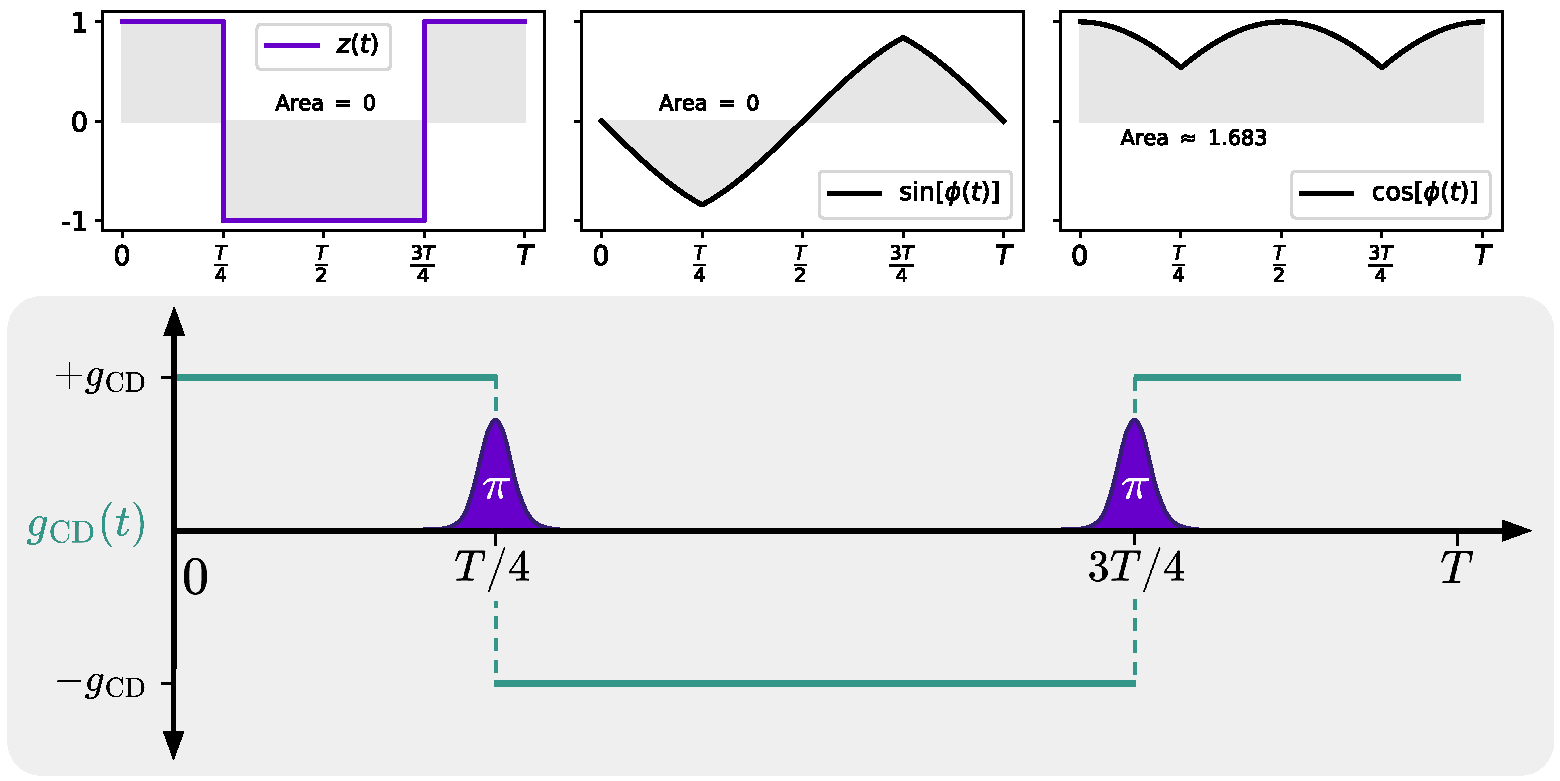
\includegraphics[width=\linewidth]{Figures/5/double_echo_FCD.pdf}
    \caption{FCD pulse implementation using the double-echo $\pi$-pulse schedule $z(t)$. Top row: numerical example of $z(t)$, $\sin[\phi(t)]$, and $\cos[\phi(t)]$ for $T = 2$ and $\chi = 4$. Observe $z(t)$ has an integral of zero as required. By modulating $g_{\rm CD}(t)$ to match the time-dependence of $z(t)$, we get constant $g_{\rm CD}(t)z(t) = 1$. The areas under $\sin[\phi(t)]$ and $\cos[\phi(t)]$ then give the relative magnitudes of the unconditional and conditional displacement rates in the FCD unitary. Bottom row: full ideal FCD pulse sequence showing the $\pi$-pulses and $g_{\rm CD}(t)$.}
    \label{fig:5_double_echo_FCD}
\end{figure}



\subsection*{Why not the RAT?}

\todo{Finish this section and comment on it}
% We numerically checked now with the full and saw that terms echo away. 
% Cancellation tone likely needed??? 

 \clearpage
 %%%%%%%%%%%%%%%%%%%%%%%%

\section{The Resonator-ATS-Fluxonium (RAF) Experiment \label{sec:5_RAF}}

\section{The 2D Dispersive Design: Moving 3D \texorpdfstring{$\to$}{to} 2D\label{sec:5_2D_Disp}}

Our final proposed approach to implement GKP error correction in 2D is our so-called 2D dispersive project. We came up with this approach during the penultimate stage of design for the RAF, which also coincided with our last attempts to fix the storage coherence issues in our 3D dispersive experiment (these issues turned out to be inherent to our 3D package). Given the daunting possibility of having to redesign the 3D experiment from scratch this late into the project, we set out to identify as many alternative paths forward as possible, and ultimately settled on the following: why not move the dispersive coupling experiment entirely to 2D, replacing the 3D cavity with an on-chip resonator? 

Of course, as we saw in the previous section, 2D resonators have higher single-photon loss rates. However, given our strategy of using a large gap low-frequency resonator in the RAF, it seems within the realm of possibility to get a storage resonator with a lifetime of $T_1 \simeq 100$ $\mu$s. As we will see below, this would already be enough to demonstrate QEC. Additionally, the idea of moving the dispersive project to 2D is attractive for several other reasons: 
\begin{enumerate}
    \item In 2D, the storage resonator and fluxonium can be directly coupled capacitively and thus we would not need an antenna to mediate the coupling. This would also eliminate the parasitic Purcell resonances that we saw in  Sec. \ref{sec:4_fluxonium_T1}.
\end{enumerate}



(1) 


This idea was very attractive for several reasons. 


why not move the entire 3D dispersive coupling experiment to 2D? 



if we can fabricate a high-coherence 2D resonator, why 


we brainstormed various avenues 


we instead arrived at a 


In order to proceed, we ultimately arrived at the following conclusion: 


We were at this point faced with the daunting engineering challenge of somehow making a 3D design 


possibility of a daunting engineering challenge to make a robust 3D design 

our options 


associated with implementing a robust 3D design, we arrived 


This approach was conceived during the last stages of design for the RAF, which also coincided 


rather quickly, as we went from ideation to a completed design in under two months


over the course of two months

This approach was developed during the final design stages of the RAF, which also coincided with 

